\documentclass[1p]{elsarticle_modified}
%\bibliographystyle{elsarticle-num}

%\usepackage[colorlinks]{hyperref}
%\usepackage{abbrmath_seonhwa} %\Abb, \Ascr, \Acal ,\Abf, \Afrak
\usepackage{amsfonts}
\usepackage{amssymb}
\usepackage{amsmath}
\usepackage{amsthm}
\usepackage{scalefnt}
\usepackage{amsbsy}
\usepackage{kotex}
\usepackage{caption}
\usepackage{subfig}
\usepackage{color}
\usepackage{graphicx}
\usepackage{xcolor} %% white, black, red, green, blue, cyan, magenta, yellow
\usepackage{float}
\usepackage{setspace}
\usepackage{hyperref}

\usepackage{tikz}
\usetikzlibrary{arrows}

\usepackage{multirow}
\usepackage{array} % fixed length table
\usepackage{hhline}

%%%%%%%%%%%%%%%%%%%%%
\makeatletter
\renewcommand*\env@matrix[1][\arraystretch]{%
	\edef\arraystretch{#1}%
	\hskip -\arraycolsep
	\let\@ifnextchar\new@ifnextchar
	\array{*\c@MaxMatrixCols c}}
\makeatother %https://tex.stackexchange.com/questions/14071/how-can-i-increase-the-line-spacing-in-a-matrix
%%%%%%%%%%%%%%%

\usepackage[normalem]{ulem}

\newcommand{\msout}[1]{\ifmmode\text{\sout{\ensuremath{#1}}}\else\sout{#1}\fi}
%SOURCE: \msout is \stkout macro in https://tex.stackexchange.com/questions/20609/strikeout-in-math-mode

\newcommand{\cancel}[1]{
	\ifmmode
	{\color{red}\msout{#1}}
	\else
	{\color{red}\sout{#1}}
	\fi
}

\newcommand{\add}[1]{
	{\color{blue}\uwave{#1}}
}

\newcommand{\replace}[2]{
	\ifmmode
	{\color{red}\msout{#1}}{\color{blue}\uwave{#2}}
	\else
	{\color{red}\sout{#1}}{\color{blue}\uwave{#2}}
	\fi
}

\newcommand{\Sol}{\mathcal{S}} %segment
\newcommand{\D}{D} %diagram
\newcommand{\A}{\mathcal{A}} %arc


%%%%%%%%%%%%%%%%%%%%%%%%%%%%%5 test

\def\sl{\operatorname{\textup{SL}}(2,\Cbb)}
\def\psl{\operatorname{\textup{PSL}}(2,\Cbb)}
\def\quan{\mkern 1mu \triangleright \mkern 1mu}

\theoremstyle{definition}
\newtheorem{thm}{Theorem}[section]
\newtheorem{prop}[thm]{Proposition}
\newtheorem{lem}[thm]{Lemma}
\newtheorem{ques}[thm]{Question}
\newtheorem{cor}[thm]{Corollary}
\newtheorem{defn}[thm]{Definition}
\newtheorem{exam}[thm]{Example}
\newtheorem{rmk}[thm]{Remark}
\newtheorem{alg}[thm]{Algorithm}

\newcommand{\I}{\sqrt{-1}}
\begin{document}

%\begin{frontmatter}
%
%\title{Boundary parabolic representations of knots up to 8 crossings}
%
%%% Group authors per affiliation:
%\author{Yunhi Cho} 
%\address{Department of Mathematics, University of Seoul, Seoul, Korea}
%\ead{yhcho@uos.ac.kr}
%
%
%\author{Seonhwa Kim} %\fnref{s_kim}}
%\address{Center for Geometry and Physics, Institute for Basic Science, Pohang, 37673, Korea}
%\ead{ryeona17@ibs.re.kr}
%
%\author{Hyuk Kim}
%\address{Department of Mathematical Sciences, Seoul National University, Seoul 08826, Korea}
%\ead{hyukkim@snu.ac.kr}
%
%\author{Seokbeom Yoon}
%\address{Department of Mathematical Sciences, Seoul National University, Seoul, 08826,  Korea}
%\ead{sbyoon15@snu.ac.kr}
%
%\begin{abstract}
%We find all boundary parabolic representation of knots up to 8 crossings.
%
%\end{abstract}
%\begin{keyword}
%    \MSC[2010] 57M25 
%\end{keyword}
%
%\end{frontmatter}

%\linenumbers
%\tableofcontents
%
\newcommand\colored[1]{\textcolor{white}{\rule[-0.35ex]{0.8em}{1.4ex}}\kern-0.8em\color{red} #1}%
%\newcommand\colored[1]{\textcolor{white}{ #1}\kern-2.17ex	\textcolor{white}{ #1}\kern-1.81ex	\textcolor{white}{ #1}\kern-2.15ex\color{red}#1	}

{\Large $\underline{12n_{0369}~(K12n_{0369})}$}

\setlength{\tabcolsep}{10pt}
\renewcommand{\arraystretch}{1.6}
\vspace{1cm}\begin{tabular}{m{100pt}>{\centering\arraybackslash}m{274pt}}
\multirow{5}{120pt}{
	\centering
	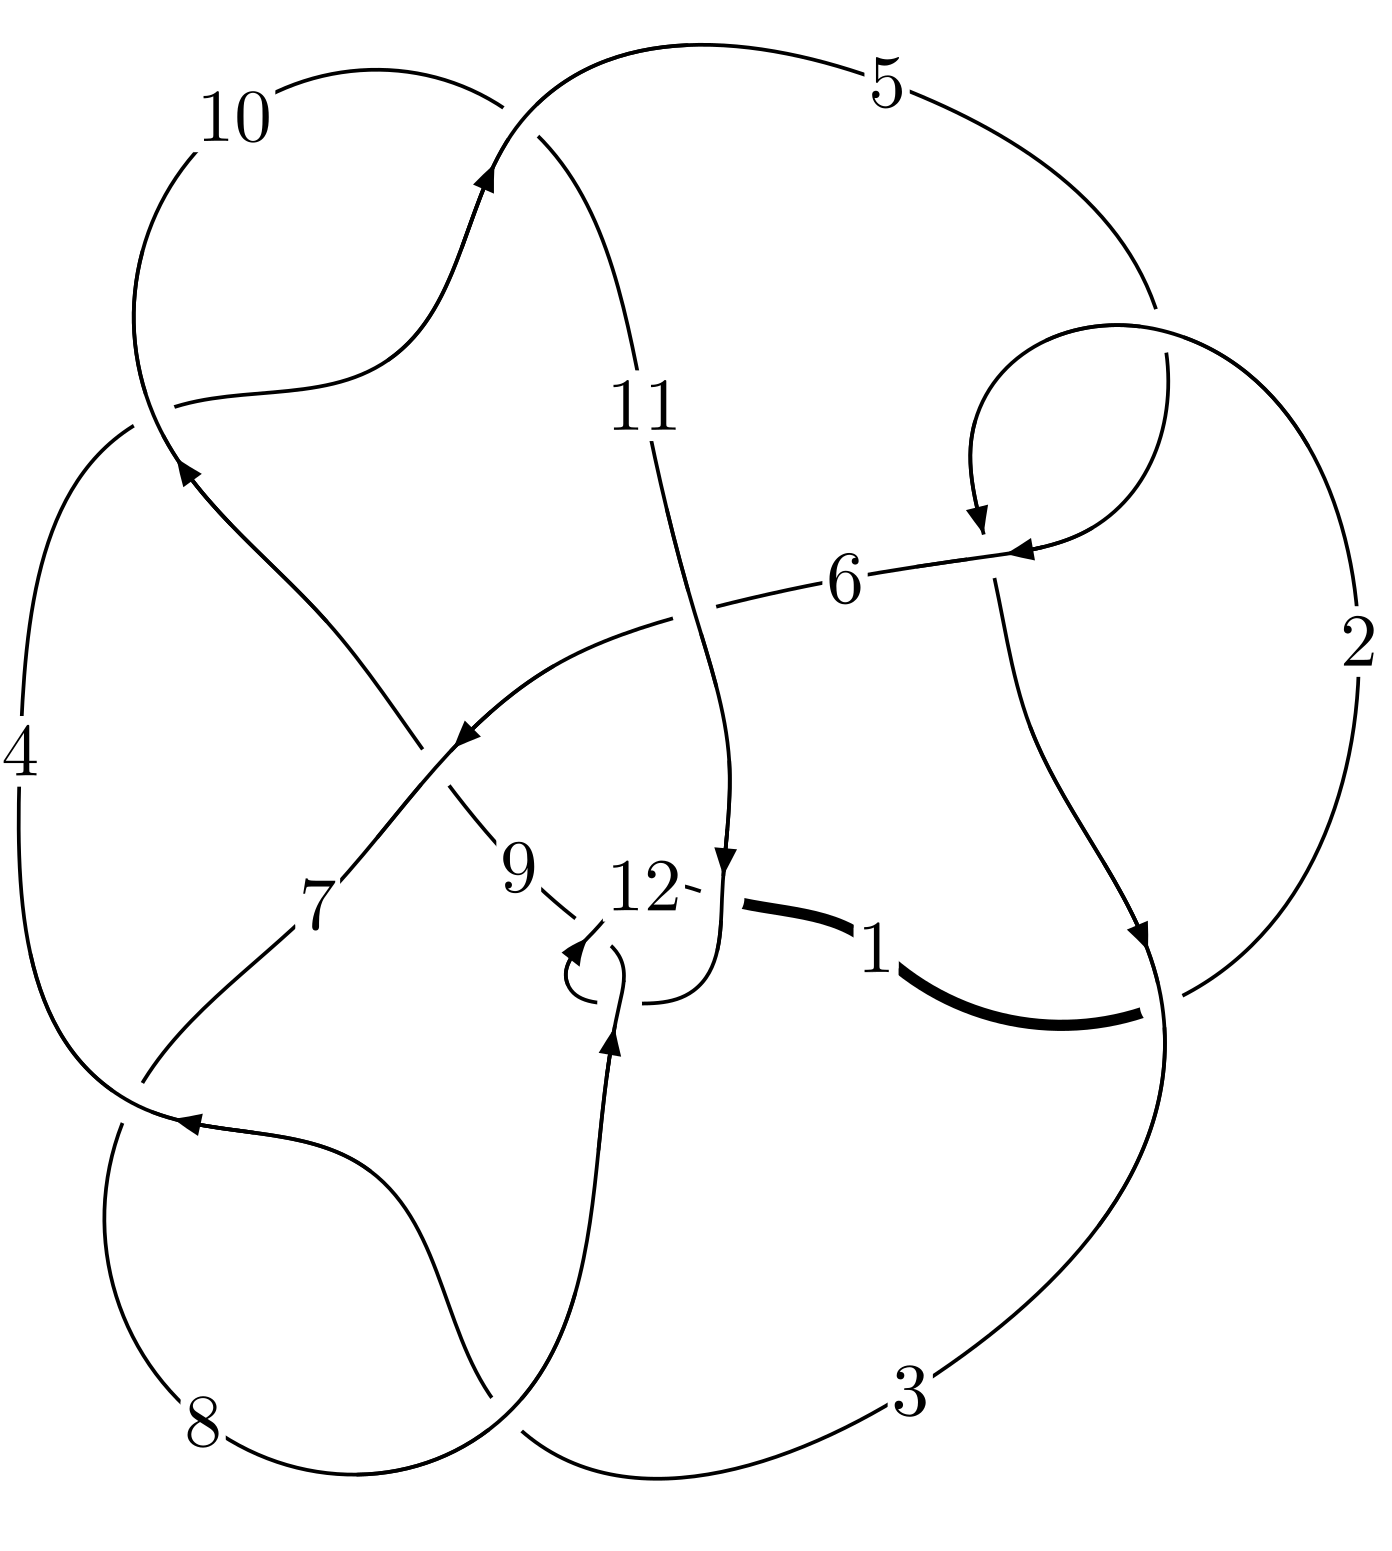
\includegraphics[width=112pt]{../../../GIT/diagram.site/Diagrams/png/2458_12n_0369.png}\\
\ \ \ A knot diagram\footnotemark}&
\allowdisplaybreaks
\textbf{Linearized knot diagam} \\
\cline{2-2}
 &
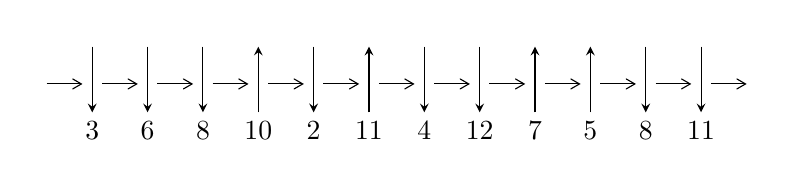
\begin{tikzpicture}[x=20pt, y=17pt]
	% nodes
	\node (C0) at (0, 0) {};
	\node (C1) at (1, 0) {};
	\node (C1U) at (1, +1) {};
	\node (C1D) at (1, -1) {3};

	\node (C2) at (2, 0) {};
	\node (C2U) at (2, +1) {};
	\node (C2D) at (2, -1) {6};

	\node (C3) at (3, 0) {};
	\node (C3U) at (3, +1) {};
	\node (C3D) at (3, -1) {8};

	\node (C4) at (4, 0) {};
	\node (C4U) at (4, +1) {};
	\node (C4D) at (4, -1) {10};

	\node (C5) at (5, 0) {};
	\node (C5U) at (5, +1) {};
	\node (C5D) at (5, -1) {2};

	\node (C6) at (6, 0) {};
	\node (C6U) at (6, +1) {};
	\node (C6D) at (6, -1) {11};

	\node (C7) at (7, 0) {};
	\node (C7U) at (7, +1) {};
	\node (C7D) at (7, -1) {4};

	\node (C8) at (8, 0) {};
	\node (C8U) at (8, +1) {};
	\node (C8D) at (8, -1) {12};

	\node (C9) at (9, 0) {};
	\node (C9U) at (9, +1) {};
	\node (C9D) at (9, -1) {7};

	\node (C10) at (10, 0) {};
	\node (C10U) at (10, +1) {};
	\node (C10D) at (10, -1) {5};

	\node (C11) at (11, 0) {};
	\node (C11U) at (11, +1) {};
	\node (C11D) at (11, -1) {8};

	\node (C12) at (12, 0) {};
	\node (C12U) at (12, +1) {};
	\node (C12D) at (12, -1) {11};
	\node (C13) at (13, 0) {};

	% arrows
	\draw[->,>={angle 60}]
	(C0) edge (C1) (C1) edge (C2) (C2) edge (C3) (C3) edge (C4) (C4) edge (C5) (C5) edge (C6) (C6) edge (C7) (C7) edge (C8) (C8) edge (C9) (C9) edge (C10) (C10) edge (C11) (C11) edge (C12) (C12) edge (C13) ;	\draw[->,>=stealth]
	(C1U) edge (C1D) (C2U) edge (C2D) (C3U) edge (C3D) (C4D) edge (C4U) (C5U) edge (C5D) (C6D) edge (C6U) (C7U) edge (C7D) (C8U) edge (C8D) (C9D) edge (C9U) (C10D) edge (C10U) (C11U) edge (C11D) (C12U) edge (C12D) ;
	\end{tikzpicture} \\
\hhline{~~} \\& 
\textbf{Solving Sequence} \\ \cline{2-2} 
 &
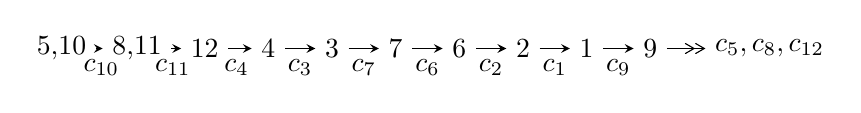
\begin{tikzpicture}[x=23pt, y=7pt]
	% node
	\node (A0) at (-1/8, 0) {5,10};
	\node (A1) at (17/16, 0) {8,11};
	\node (A2) at (17/8, 0) {12};
	\node (A3) at (25/8, 0) {4};
	\node (A4) at (33/8, 0) {3};
	\node (A5) at (41/8, 0) {7};
	\node (A6) at (49/8, 0) {6};
	\node (A7) at (57/8, 0) {2};
	\node (A8) at (65/8, 0) {1};
	\node (A9) at (73/8, 0) {9};
	\node (C1) at (1/2, -1) {$c_{10}$};
	\node (C2) at (13/8, -1) {$c_{11}$};
	\node (C3) at (21/8, -1) {$c_{4}$};
	\node (C4) at (29/8, -1) {$c_{3}$};
	\node (C5) at (37/8, -1) {$c_{7}$};
	\node (C6) at (45/8, -1) {$c_{6}$};
	\node (C7) at (53/8, -1) {$c_{2}$};
	\node (C8) at (61/8, -1) {$c_{1}$};
	\node (C9) at (69/8, -1) {$c_{9}$};
	\node (A10) at (11, 0) {$c_{5},c_{8},c_{12}$};

	% edge
	\draw[->,>=stealth]	
	(A0) edge (A1) (A1) edge (A2) (A2) edge (A3) (A3) edge (A4) (A4) edge (A5) (A5) edge (A6) (A6) edge (A7) (A7) edge (A8) (A8) edge (A9) ;
	\draw[->>,>={angle 60}]	
	(A9) edge (A10);
\end{tikzpicture} \\ 

\end{tabular} \\

\footnotetext{
The image of knot diagram is generated by the software ``\textbf{Draw programme}" developed by Andrew Bartholomew(\url{http://www.layer8.co.uk/maths/draw/index.htm\#Running-draw}), where we modified some parts for our purpose(\url{https://github.com/CATsTAILs/LinksPainter}).
}\phantom \\ \newline 
\centering \textbf{Ideals for irreducible components\footnotemark of $X_{\text{par}}$} 
 
\begin{align*}
I^u_{1}&=\langle 
-2.75957\times10^{30} u^{47}+3.57679\times10^{30} u^{46}+\cdots+6.32723\times10^{30} b-3.65231\times10^{30},\\
\phantom{I^u_{1}}&\phantom{= \langle  }-2.09830\times10^{31} u^{47}-2.86459\times10^{31} u^{46}+\cdots+6.32723\times10^{30} a+1.84790\times10^{32},\;u^{48}+u^{47}+\cdots-10 u+1\rangle \\
I^u_{2}&=\langle 
u^{14}-7 u^{12}+u^{11}+17 u^{10}-6 u^9-12 u^8+12 u^7-13 u^6-8 u^5+17 u^4- u^3+u^2+b+u,\\
\phantom{I^u_{2}}&\phantom{= \langle  }- u^{15}-2 u^{14}+\cdots+a+1,\\
\phantom{I^u_{2}}&\phantom{= \langle  }u^{16}-8 u^{14}+u^{13}+25 u^{12}-7 u^{11}-34 u^{10}+19 u^9+7 u^8-24 u^7+30 u^6+12 u^5-25 u^4+u^3+2 u^2-2 u+1\rangle \\
I^u_{3}&=\langle 
b,\;a-1,\;u^4- u^3-1\rangle \\
I^u_{4}&=\langle 
b,\;a-1,\;u+1\rangle \\
\\
\end{align*}
\raggedright * 4 irreducible components of $\dim_{\mathbb{C}}=0$, with total 69 representations.\\
\footnotetext{All coefficients of polynomials are rational numbers. But the coefficients are sometimes approximated in decimal forms when there is not enough margin.}
\newpage
\renewcommand{\arraystretch}{1}
\centering \section*{I. $I^u_{1}= \langle -2.76\times10^{30} u^{47}+3.58\times10^{30} u^{46}+\cdots+6.33\times10^{30} b-3.65\times10^{30},\;-2.10\times10^{31} u^{47}-2.86\times10^{31} u^{46}+\cdots+6.33\times10^{30} a+1.85\times10^{32},\;u^{48}+u^{47}+\cdots-10 u+1 \rangle$}
\flushleft \textbf{(i) Arc colorings}\\
\begin{tabular}{m{7pt} m{180pt} m{7pt} m{180pt} }
\flushright $a_{5}=$&$\begin{pmatrix}0\\u\end{pmatrix}$ \\
\flushright $a_{10}=$&$\begin{pmatrix}1\\0\end{pmatrix}$ \\
\flushright $a_{8}=$&$\begin{pmatrix}3.31630 u^{47}+4.52741 u^{46}+\cdots+38.4903 u-29.2055\\0.436142 u^{47}-0.565302 u^{46}+\cdots+1.59289 u+0.577237\end{pmatrix}$ \\
\flushright $a_{11}=$&$\begin{pmatrix}1\\- u^2\end{pmatrix}$ \\
\flushright $a_{12}=$&$\begin{pmatrix}0.242854 u^{47}+2.03129 u^{46}+\cdots+69.3445 u-20.8066\\1.64294 u^{47}+0.0993437 u^{46}+\cdots-21.2574 u+1.65185\end{pmatrix}$ \\
\flushright $a_{4}=$&$\begin{pmatrix}- u\\u\end{pmatrix}$ \\
\flushright $a_{3}=$&$\begin{pmatrix}-1.28265 u^{47}-0.830559 u^{46}+\cdots-36.6527 u-1.12768\\0.892123 u^{47}+0.107793 u^{46}+\cdots-6.10035 u-1.43370\end{pmatrix}$ \\
\flushright $a_{7}=$&$\begin{pmatrix}3.37390 u^{47}+4.39684 u^{46}+\cdots+36.8345 u-29.4151\\0.378539 u^{47}-0.434740 u^{46}+\cdots+3.24866 u+0.786904\end{pmatrix}$ \\
\flushright $a_{6}=$&$\begin{pmatrix}3.76580 u^{47}+4.48846 u^{46}+\cdots+26.7303 u-29.1791\\-0.222098 u^{47}-0.473962 u^{46}+\cdots+6.64344 u+0.486616\end{pmatrix}$ \\
\flushright $a_{2}=$&$\begin{pmatrix}2.90620 u^{47}+2.89459 u^{46}+\cdots-5.12037 u-23.2385\\0.210719 u^{47}+0.258112 u^{46}+\cdots+7.62863 u-0.669658\end{pmatrix}$ \\
\flushright $a_{1}=$&$\begin{pmatrix}-0.607997 u^{47}-1.69785 u^{46}+\cdots-72.9604 u+20.6700\\-0.837878 u^{47}-0.317904 u^{46}+\cdots+13.9065 u-0.953269\end{pmatrix}$ \\
\flushright $a_{9}=$&$\begin{pmatrix}3.59091 u^{47}+1.91005 u^{46}+\cdots+69.2709 u-21.1928\\-1.82497 u^{47}+0.418307 u^{46}+\cdots-0.762950 u+0.364889\end{pmatrix}$\\&\end{tabular}
\flushleft \textbf{(ii) Obstruction class $= -1$}\\~\\
\flushleft \textbf{(iii) Cusp Shapes $= -2.37527 u^{47}-1.29990 u^{46}+\cdots+83.9395 u+0.965224$}\\~\\
\newpage\renewcommand{\arraystretch}{1}
\flushleft \textbf{(iv) u-Polynomials at the component}\newline \\
\begin{tabular}{m{50pt}|m{274pt}}
Crossings & \hspace{64pt}u-Polynomials at each crossing \\
\hline $$\begin{aligned}c_{1}\end{aligned}$$&$\begin{aligned}
&u^{48}+30 u^{47}+\cdots+204 u+16
\end{aligned}$\\
\hline $$\begin{aligned}c_{2},c_{5}\end{aligned}$$&$\begin{aligned}
&u^{48}-4 u^{47}+\cdots-34 u+4
\end{aligned}$\\
\hline $$\begin{aligned}c_{3},c_{7}\end{aligned}$$&$\begin{aligned}
&u^{48}+2 u^{47}+\cdots-16 u+1
\end{aligned}$\\
\hline $$\begin{aligned}c_{4},c_{10}\end{aligned}$$&$\begin{aligned}
&u^{48}+u^{47}+\cdots-10 u+1
\end{aligned}$\\
\hline $$\begin{aligned}c_{6}\end{aligned}$$&$\begin{aligned}
&u^{48}+3 u^{47}+\cdots-18570 u+68953
\end{aligned}$\\
\hline $$\begin{aligned}c_{8},c_{11}\end{aligned}$$&$\begin{aligned}
&u^{48}+5 u^{47}+\cdots+120 u+271
\end{aligned}$\\
\hline $$\begin{aligned}c_{9}\end{aligned}$$&$\begin{aligned}
&u^{48}+11 u^{47}+\cdots+46158 u+10853
\end{aligned}$\\
\hline $$\begin{aligned}c_{12}\end{aligned}$$&$\begin{aligned}
&u^{48}+59 u^{47}+\cdots+2718438 u+73441
\end{aligned}$\\
\hline
\end{tabular}\\~\\
\newpage\renewcommand{\arraystretch}{1}
\flushleft \textbf{(v) Riley Polynomials at the component}\newline \\
\begin{tabular}{m{50pt}|m{274pt}}
Crossings & \hspace{64pt}Riley Polynomials at each crossing \\
\hline $$\begin{aligned}c_{1}\end{aligned}$$&$\begin{aligned}
&y^{48}-18 y^{47}+\cdots-209520 y+256
\end{aligned}$\\
\hline $$\begin{aligned}c_{2},c_{5}\end{aligned}$$&$\begin{aligned}
&y^{48}-30 y^{47}+\cdots-204 y+16
\end{aligned}$\\
\hline $$\begin{aligned}c_{3},c_{7}\end{aligned}$$&$\begin{aligned}
&y^{48}+10 y^{47}+\cdots-162 y+1
\end{aligned}$\\
\hline $$\begin{aligned}c_{4},c_{10}\end{aligned}$$&$\begin{aligned}
&y^{48}-43 y^{47}+\cdots-166 y+1
\end{aligned}$\\
\hline $$\begin{aligned}c_{6}\end{aligned}$$&$\begin{aligned}
&y^{48}+25 y^{47}+\cdots-20064851276 y+4754516209
\end{aligned}$\\
\hline $$\begin{aligned}c_{8},c_{11}\end{aligned}$$&$\begin{aligned}
&y^{48}-59 y^{47}+\cdots-2718438 y+73441
\end{aligned}$\\
\hline $$\begin{aligned}c_{9}\end{aligned}$$&$\begin{aligned}
&y^{48}+5 y^{47}+\cdots-97685534 y+117787609
\end{aligned}$\\
\hline $$\begin{aligned}c_{12}\end{aligned}$$&$\begin{aligned}
&y^{48}-143 y^{47}+\cdots-163732164302 y+5393580481
\end{aligned}$\\
\hline
\end{tabular}\\~\\
\newpage\flushleft \textbf{(vi) Complex Volumes and Cusp Shapes}
$$\begin{array}{c|c|c}  
\text{Solutions to }I^u_{1}& \I (\text{vol} + \sqrt{-1}CS) & \text{Cusp shape}\\
 \hline 
\begin{aligned}
u &= \phantom{-}0.188816 + 0.986534 I \\
a &= -1.187120 - 0.629861 I \\
b &= \phantom{-}0.344371 - 0.579813 I\end{aligned}
 & -11.1663 + 9.4251 I & -7.81565 - 5.65269 I \\ \hline\begin{aligned}
u &= \phantom{-}0.188816 - 0.986534 I \\
a &= -1.187120 + 0.629861 I \\
b &= \phantom{-}0.344371 + 0.579813 I\end{aligned}
 & -11.1663 - 9.4251 I & -7.81565 + 5.65269 I \\ \hline\begin{aligned}
u &= -0.923856\phantom{ +0.000000I} \\
a &= \phantom{-}0.987425\phantom{ +0.000000I} \\
b &= -0.00645573\phantom{ +0.000000I}\end{aligned}
 & -1.64390\phantom{ +0.000000I} & -6.03810\phantom{ +0.000000I} \\ \hline\begin{aligned}
u &= -0.118797 + 0.851176 I \\
a &= -1.42725 + 0.86776 I \\
b &= \phantom{-}0.414622 + 0.529642 I\end{aligned}
 & -7.00819 - 3.87744 I & -6.00183 + 2.83114 I \\ \hline\begin{aligned}
u &= -0.118797 - 0.851176 I \\
a &= -1.42725 - 0.86776 I \\
b &= \phantom{-}0.414622 - 0.529642 I\end{aligned}
 & -7.00819 + 3.87744 I & -6.00183 - 2.83114 I \\ \hline\begin{aligned}
u &= -0.237043 + 0.810777 I \\
a &= \phantom{-}0.266448 - 0.209284 I \\
b &= -0.484219 - 0.035427 I\end{aligned}
 & -1.59052 + 1.65508 I & -10.14529 - 5.18915 I \\ \hline\begin{aligned}
u &= -0.237043 - 0.810777 I \\
a &= \phantom{-}0.266448 + 0.209284 I \\
b &= -0.484219 + 0.035427 I\end{aligned}
 & -1.59052 - 1.65508 I & -10.14529 + 5.18915 I \\ \hline\begin{aligned}
u &= -0.058232 + 0.837894 I \\
a &= -1.82697 - 0.63370 I \\
b &= \phantom{-}0.516515 - 0.576658 I\end{aligned}
 & -11.32710 - 1.67337 I & -8.90827 + 0.94865 I \\ \hline\begin{aligned}
u &= -0.058232 - 0.837894 I \\
a &= -1.82697 + 0.63370 I \\
b &= \phantom{-}0.516515 + 0.576658 I\end{aligned}
 & -11.32710 + 1.67337 I & -8.90827 - 0.94865 I \\ \hline\begin{aligned}
u &= -1.147810 + 0.393065 I \\
a &= \phantom{-}0.063356 - 0.460733 I \\
b &= -1.191290 + 0.713713 I\end{aligned}
 & -3.86248 - 0.61447 I & \phantom{-0.000000 } 0\\
 \hline 
 \end{array}$$\newpage$$\begin{array}{c|c|c}  
\text{Solutions to }I^u_{1}& \I (\text{vol} + \sqrt{-1}CS) & \text{Cusp shape}\\
 \hline 
\begin{aligned}
u &= -1.147810 - 0.393065 I \\
a &= \phantom{-}0.063356 + 0.460733 I \\
b &= -1.191290 - 0.713713 I\end{aligned}
 & -3.86248 + 0.61447 I & \phantom{-0.000000 } 0 \\ \hline\begin{aligned}
u &= \phantom{-}1.224880 + 0.039706 I \\
a &= -0.84589 + 2.01472 I \\
b &= \phantom{-}0.75845 - 3.13225 I\end{aligned}
 & \phantom{-}5.47066 + 2.81993 I & \phantom{-0.000000 } 0 \\ \hline\begin{aligned}
u &= \phantom{-}1.224880 - 0.039706 I \\
a &= -0.84589 - 2.01472 I \\
b &= \phantom{-}0.75845 + 3.13225 I\end{aligned}
 & \phantom{-}5.47066 - 2.81993 I & \phantom{-0.000000 } 0 \\ \hline\begin{aligned}
u &= -1.23724\phantom{ +0.000000I} \\
a &= \phantom{-}3.88112\phantom{ +0.000000I} \\
b &= -3.94762\phantom{ +0.000000I}\end{aligned}
 & -3.66178\phantom{ +0.000000I} & \phantom{-}3.85220\phantom{ +0.000000I} \\ \hline\begin{aligned}
u &= -0.228880 + 0.722151 I \\
a &= \phantom{-}0.583716 - 0.181097 I \\
b &= -0.334046 - 0.976538 I\end{aligned}
 & -3.67584 - 3.60264 I & -9.48140 + 6.24040 I \\ \hline\begin{aligned}
u &= -0.228880 - 0.722151 I \\
a &= \phantom{-}0.583716 + 0.181097 I \\
b &= -0.334046 + 0.976538 I\end{aligned}
 & -3.67584 + 3.60264 I & -9.48140 - 6.24040 I \\ \hline\begin{aligned}
u &= \phantom{-}1.178910 + 0.418615 I \\
a &= -0.475538 - 0.859997 I \\
b &= \phantom{-}0.42509 + 1.83991 I\end{aligned}
 & \phantom{-}1.37240 + 4.77913 I & \phantom{-0.000000 } 0 \\ \hline\begin{aligned}
u &= \phantom{-}1.178910 - 0.418615 I \\
a &= -0.475538 + 0.859997 I \\
b &= \phantom{-}0.42509 - 1.83991 I\end{aligned}
 & \phantom{-}1.37240 - 4.77913 I & \phantom{-0.000000 } 0 \\ \hline\begin{aligned}
u &= -1.211720 + 0.403316 I \\
a &= \phantom{-}0.412396 + 0.097054 I \\
b &= -0.007786 + 0.341023 I\end{aligned}
 & \phantom{-}1.52928 - 6.15730 I & \phantom{-0.000000 } 0 \\ \hline\begin{aligned}
u &= -1.211720 - 0.403316 I \\
a &= \phantom{-}0.412396 - 0.097054 I \\
b &= -0.007786 - 0.341023 I\end{aligned}
 & \phantom{-}1.52928 + 6.15730 I & \phantom{-0.000000 } 0\\
 \hline 
 \end{array}$$\newpage$$\begin{array}{c|c|c}  
\text{Solutions to }I^u_{1}& \I (\text{vol} + \sqrt{-1}CS) & \text{Cusp shape}\\
 \hline 
\begin{aligned}
u &= \phantom{-}1.260750 + 0.217181 I \\
a &= \phantom{-}0.580734 + 0.080863 I \\
b &= -0.153480 - 0.378533 I\end{aligned}
 & \phantom{-}3.26609 + 1.25196 I & \phantom{-0.000000 } 0 \\ \hline\begin{aligned}
u &= \phantom{-}1.260750 - 0.217181 I \\
a &= \phantom{-}0.580734 - 0.080863 I \\
b &= -0.153480 + 0.378533 I\end{aligned}
 & \phantom{-}3.26609 - 1.25196 I & \phantom{-0.000000 } 0 \\ \hline\begin{aligned}
u &= -1.228180 + 0.379942 I \\
a &= \phantom{-}0.05711 - 2.29319 I \\
b &= \phantom{-}0.30107 + 3.26878 I\end{aligned}
 & -7.72334 - 2.70340 I & \phantom{-0.000000 } 0 \\ \hline\begin{aligned}
u &= -1.228180 - 0.379942 I \\
a &= \phantom{-}0.05711 + 2.29319 I \\
b &= \phantom{-}0.30107 - 3.26878 I\end{aligned}
 & -7.72334 + 2.70340 I & \phantom{-0.000000 } 0 \\ \hline\begin{aligned}
u &= -1.289200 + 0.073390 I \\
a &= -0.63077 + 1.65237 I \\
b &= \phantom{-}0.35618 - 2.71369 I\end{aligned}
 & \phantom{-}6.48354 - 3.11664 I & \phantom{-0.000000 } 0 \\ \hline\begin{aligned}
u &= -1.289200 - 0.073390 I \\
a &= -0.63077 - 1.65237 I \\
b &= \phantom{-}0.35618 + 2.71369 I\end{aligned}
 & \phantom{-}6.48354 + 3.11664 I & \phantom{-0.000000 } 0 \\ \hline\begin{aligned}
u &= \phantom{-}1.154930 + 0.634373 I \\
a &= -0.078971 + 0.444060 I \\
b &= -0.849057 - 0.707892 I\end{aligned}
 & -8.27166 - 3.77639 I & \phantom{-0.000000 } 0 \\ \hline\begin{aligned}
u &= \phantom{-}1.154930 - 0.634373 I \\
a &= -0.078971 - 0.444060 I \\
b &= -0.849057 + 0.707892 I\end{aligned}
 & -8.27166 + 3.77639 I & \phantom{-0.000000 } 0 \\ \hline\begin{aligned}
u &= \phantom{-}1.319420 + 0.377715 I \\
a &= \phantom{-}0.051061 + 0.623648 I \\
b &= -1.16317 - 1.04567 I\end{aligned}
 & -7.01248 + 6.04669 I & \phantom{-0.000000 } 0 \\ \hline\begin{aligned}
u &= \phantom{-}1.319420 - 0.377715 I \\
a &= \phantom{-}0.051061 - 0.623648 I \\
b &= -1.16317 + 1.04567 I\end{aligned}
 & -7.01248 - 6.04669 I & \phantom{-0.000000 } 0\\
 \hline 
 \end{array}$$\newpage$$\begin{array}{c|c|c}  
\text{Solutions to }I^u_{1}& \I (\text{vol} + \sqrt{-1}CS) & \text{Cusp shape}\\
 \hline 
\begin{aligned}
u &= -0.612128\phantom{ +0.000000I} \\
a &= -0.328856\phantom{ +0.000000I} \\
b &= -1.19564\phantom{ +0.000000I}\end{aligned}
 & -2.95942\phantom{ +0.000000I} & \phantom{-}2.44780\phantom{ +0.000000I} \\ \hline\begin{aligned}
u &= \phantom{-}1.353320 + 0.378263 I \\
a &= -0.08340 + 1.97303 I \\
b &= \phantom{-}0.49945 - 2.98749 I\end{aligned}
 & -2.37757 + 8.30419 I & \phantom{-0.000000 } 0 \\ \hline\begin{aligned}
u &= \phantom{-}1.353320 - 0.378263 I \\
a &= -0.08340 - 1.97303 I \\
b &= \phantom{-}0.49945 + 2.98749 I\end{aligned}
 & -2.37757 - 8.30419 I & \phantom{-0.000000 } 0 \\ \hline\begin{aligned}
u &= -1.394650 + 0.226156 I \\
a &= -0.28775 + 1.52139 I \\
b &= \phantom{-}0.01735 - 2.20388 I\end{aligned}
 & \phantom{-}4.97003 - 4.04918 I & \phantom{-0.000000 } 0 \\ \hline\begin{aligned}
u &= -1.394650 - 0.226156 I \\
a &= -0.28775 - 1.52139 I \\
b &= \phantom{-}0.01735 + 2.20388 I\end{aligned}
 & \phantom{-}4.97003 + 4.04918 I & \phantom{-0.000000 } 0 \\ \hline\begin{aligned}
u &= \phantom{-}0.204671 + 0.542777 I \\
a &= \phantom{-}0.606882 + 0.463380 I \\
b &= -0.097702 + 0.457637 I\end{aligned}
 & -0.184718 + 1.155860 I & -2.61813 - 5.93351 I \\ \hline\begin{aligned}
u &= \phantom{-}0.204671 - 0.542777 I \\
a &= \phantom{-}0.606882 - 0.463380 I \\
b &= -0.097702 - 0.457637 I\end{aligned}
 & -0.184718 - 1.155860 I & -2.61813 + 5.93351 I \\ \hline\begin{aligned}
u &= \phantom{-}1.39354 + 0.29007 I \\
a &= -0.54475 - 1.82044 I \\
b &= \phantom{-}0.09576 + 2.31209 I\end{aligned}
 & \phantom{-}1.48745 + 7.27926 I & \phantom{-0.000000 } 0 \\ \hline\begin{aligned}
u &= \phantom{-}1.39354 - 0.29007 I \\
a &= -0.54475 + 1.82044 I \\
b &= \phantom{-}0.09576 - 2.31209 I\end{aligned}
 & \phantom{-}1.48745 - 7.27926 I & \phantom{-0.000000 } 0 \\ \hline\begin{aligned}
u &= \phantom{-}1.43184 + 0.09274 I \\
a &= \phantom{-}0.510399 - 1.211730 I \\
b &= -0.44308 + 1.62054 I\end{aligned}
 & \phantom{-}4.22730 + 0.98369 I & \phantom{-0.000000 } 0\\
 \hline 
 \end{array}$$\newpage$$\begin{array}{c|c|c}  
\text{Solutions to }I^u_{1}& \I (\text{vol} + \sqrt{-1}CS) & \text{Cusp shape}\\
 \hline 
\begin{aligned}
u &= \phantom{-}1.43184 - 0.09274 I \\
a &= \phantom{-}0.510399 + 1.211730 I \\
b &= -0.44308 - 1.62054 I\end{aligned}
 & \phantom{-}4.22730 - 0.98369 I & \phantom{-0.000000 } 0 \\ \hline\begin{aligned}
u &= -1.41425 + 0.42968 I \\
a &= -0.01233 - 1.80833 I \\
b &= \phantom{-}0.45419 + 2.79557 I\end{aligned}
 & -6.1055 - 14.4818 I & \phantom{-0.000000 } 0 \\ \hline\begin{aligned}
u &= -1.41425 - 0.42968 I \\
a &= -0.01233 + 1.80833 I \\
b &= \phantom{-}0.45419 - 2.79557 I\end{aligned}
 & -6.1055 + 14.4818 I & \phantom{-0.000000 } 0 \\ \hline\begin{aligned}
u &= -1.50303 + 0.27534 I \\
a &= -0.016901 + 1.163320 I \\
b &= \phantom{-}0.04802 - 1.86187 I\end{aligned}
 & \phantom{-}4.18133 - 4.41038 I & \phantom{-0.000000 } 0 \\ \hline\begin{aligned}
u &= -1.50303 - 0.27534 I \\
a &= -0.016901 - 1.163320 I \\
b &= \phantom{-}0.04802 + 1.86187 I\end{aligned}
 & \phantom{-}4.18133 + 4.41038 I & \phantom{-0.000000 } 0 \\ \hline\begin{aligned}
u &= -0.212607\phantom{ +0.000000I} \\
a &= \phantom{-}5.78141\phantom{ +0.000000I} \\
b &= -2.13725\phantom{ +0.000000I}\end{aligned}
 & -6.86165\phantom{ +0.000000I} & -17.4210\phantom{ +0.000000I} \\ \hline\begin{aligned}
u &= \phantom{-}0.1136290 + 0.0195248 I \\
a &= -0.87499 + 10.27460 I \\
b &= \phantom{-}0.636242 + 0.063087 I\end{aligned}
 & \phantom{-}2.11273 + 2.53080 I & \phantom{-}5.85801 - 0.41014 I \\ \hline\begin{aligned}
u &= \phantom{-}0.1136290 - 0.0195248 I \\
a &= -0.87499 - 10.27460 I \\
b &= \phantom{-}0.636242 - 0.063087 I\end{aligned}
 & \phantom{-}2.11273 - 2.53080 I & \phantom{-}5.85801 + 0.41014 I\\
 \hline 
 \end{array}$$\newpage\newpage\renewcommand{\arraystretch}{1}
\centering \section*{II. $I^u_{2}= \langle u^{14}-7 u^{12}+\cdots+b+u,\;- u^{15}-2 u^{14}+\cdots+a+1,\;u^{16}-8 u^{14}+\cdots-2 u+1 \rangle$}
\flushleft \textbf{(i) Arc colorings}\\
\begin{tabular}{m{7pt} m{180pt} m{7pt} m{180pt} }
\flushright $a_{5}=$&$\begin{pmatrix}0\\u\end{pmatrix}$ \\
\flushright $a_{10}=$&$\begin{pmatrix}1\\0\end{pmatrix}$ \\
\flushright $a_{8}=$&$\begin{pmatrix}u^{15}+2 u^{14}+\cdots+4 u-1\\- u^{14}+7 u^{12}+\cdots- u^2- u\end{pmatrix}$ \\
\flushright $a_{11}=$&$\begin{pmatrix}1\\- u^2\end{pmatrix}$ \\
\flushright $a_{12}=$&$\begin{pmatrix}-2 u^{15}+4 u^{14}+\cdots+6 u-2\\u^{15}-4 u^{14}+\cdots-8 u+4\end{pmatrix}$ \\
\flushright $a_{4}=$&$\begin{pmatrix}- u\\u\end{pmatrix}$ \\
\flushright $a_{3}=$&$\begin{pmatrix}- u^{14}- u^{13}+\cdots+3 u-1\\u^{15}+u^{14}+\cdots- u^2+2 u\end{pmatrix}$ \\
\flushright $a_{7}=$&$\begin{pmatrix}u^{15}+3 u^{14}+\cdots+5 u-2\\-2 u^{14}+13 u^{12}+\cdots-2 u+1\end{pmatrix}$ \\
\flushright $a_{6}=$&$\begin{pmatrix}u^{15}+u^{14}+\cdots-6 u^2+2 u\\u^{14}-6 u^{12}+\cdots+2 u-1\end{pmatrix}$ \\
\flushright $a_{2}=$&$\begin{pmatrix}- u^{15}+6 u^{13}+\cdots-4 u^2+6 u\\2 u^{15}+2 u^{14}+\cdots+2 u^2+u\end{pmatrix}$ \\
\flushright $a_{1}=$&$\begin{pmatrix}-2 u^{15}+2 u^{14}+\cdots+4 u-2\\u^{15}- u^{14}+\cdots-4 u+2\end{pmatrix}$ \\
\flushright $a_{9}=$&$\begin{pmatrix}2 u^{15}-7 u^{14}+\cdots-9 u+6\\-2 u^{15}+6 u^{14}+\cdots+7 u-3\end{pmatrix}$\\&\end{tabular}
\flushleft \textbf{(ii) Obstruction class $= 1$}\\~\\
\flushleft \textbf{(iii) Cusp Shapes $= 6 u^{15}-3 u^{14}-39 u^{13}+23 u^{12}+89 u^{11}-65 u^{10}-52 u^9+74 u^8-90 u^7-14 u^6+120 u^5-24 u^4-7 u^3+8 u^2-21 u-8$}\\~\\
\newpage\renewcommand{\arraystretch}{1}
\flushleft \textbf{(iv) u-Polynomials at the component}\newline \\
\begin{tabular}{m{50pt}|m{274pt}}
Crossings & \hspace{64pt}u-Polynomials at each crossing \\
\hline $$\begin{aligned}c_{1}\end{aligned}$$&$\begin{aligned}
&u^{16}-10 u^{15}+\cdots-13 u+1
\end{aligned}$\\
\hline $$\begin{aligned}c_{2}\end{aligned}$$&$\begin{aligned}
&u^{16}-5 u^{14}+\cdots+u+1
\end{aligned}$\\
\hline $$\begin{aligned}c_{3}\end{aligned}$$&$\begin{aligned}
&u^{16}+u^{15}+\cdots+2 u^2+1
\end{aligned}$\\
\hline $$\begin{aligned}c_{4}\end{aligned}$$&$\begin{aligned}
&u^{16}-8 u^{14}+\cdots+2 u+1
\end{aligned}$\\
\hline $$\begin{aligned}c_{5}\end{aligned}$$&$\begin{aligned}
&u^{16}-5 u^{14}+\cdots- u+1
\end{aligned}$\\
\hline $$\begin{aligned}c_{6}\end{aligned}$$&$\begin{aligned}
&u^{16}-10 u^{14}+\cdots-8 u+1
\end{aligned}$\\
\hline $$\begin{aligned}c_{7}\end{aligned}$$&$\begin{aligned}
&u^{16}- u^{15}+\cdots+2 u^2+1
\end{aligned}$\\
\hline $$\begin{aligned}c_{8}\end{aligned}$$&$\begin{aligned}
&u^{16}+4 u^{15}+\cdots-6 u^2+1
\end{aligned}$\\
\hline $$\begin{aligned}c_{9}\end{aligned}$$&$\begin{aligned}
&u^{16}-10 u^{14}+\cdots-10 u+1
\end{aligned}$\\
\hline $$\begin{aligned}c_{10}\end{aligned}$$&$\begin{aligned}
&u^{16}-8 u^{14}+\cdots-2 u+1
\end{aligned}$\\
\hline $$\begin{aligned}c_{11}\end{aligned}$$&$\begin{aligned}
&u^{16}-4 u^{15}+\cdots-6 u^2+1
\end{aligned}$\\
\hline $$\begin{aligned}c_{12}\end{aligned}$$&$\begin{aligned}
&u^{16}+16 u^{15}+\cdots+12 u+1
\end{aligned}$\\
\hline
\end{tabular}\\~\\
\newpage\renewcommand{\arraystretch}{1}
\flushleft \textbf{(v) Riley Polynomials at the component}\newline \\
\begin{tabular}{m{50pt}|m{274pt}}
Crossings & \hspace{64pt}Riley Polynomials at each crossing \\
\hline $$\begin{aligned}c_{1}\end{aligned}$$&$\begin{aligned}
&y^{16}+2 y^{15}+\cdots-17 y+1
\end{aligned}$\\
\hline $$\begin{aligned}c_{2},c_{5}\end{aligned}$$&$\begin{aligned}
&y^{16}-10 y^{15}+\cdots-13 y+1
\end{aligned}$\\
\hline $$\begin{aligned}c_{3},c_{7}\end{aligned}$$&$\begin{aligned}
&y^{16}+9 y^{15}+\cdots+4 y+1
\end{aligned}$\\
\hline $$\begin{aligned}c_{4},c_{10}\end{aligned}$$&$\begin{aligned}
&y^{16}-16 y^{15}+\cdots-42 y^2+1
\end{aligned}$\\
\hline $$\begin{aligned}c_{6}\end{aligned}$$&$\begin{aligned}
&y^{16}-20 y^{15}+\cdots-26 y+1
\end{aligned}$\\
\hline $$\begin{aligned}c_{8},c_{11}\end{aligned}$$&$\begin{aligned}
&y^{16}-16 y^{15}+\cdots-12 y+1
\end{aligned}$\\
\hline $$\begin{aligned}c_{9}\end{aligned}$$&$\begin{aligned}
&y^{16}-20 y^{15}+\cdots-28 y+1
\end{aligned}$\\
\hline $$\begin{aligned}c_{12}\end{aligned}$$&$\begin{aligned}
&y^{16}-36 y^{15}+\cdots-16 y+1
\end{aligned}$\\
\hline
\end{tabular}\\~\\
\newpage\flushleft \textbf{(vi) Complex Volumes and Cusp Shapes}
$$\begin{array}{c|c|c}  
\text{Solutions to }I^u_{2}& \I (\text{vol} + \sqrt{-1}CS) & \text{Cusp shape}\\
 \hline 
\begin{aligned}
u &= \phantom{-}0.157905 + 0.943251 I \\
a &= \phantom{-}0.610640 + 0.247441 I \\
b &= \phantom{-}0.0788746 - 0.0514506 I\end{aligned}
 & -0.93275 - 1.38263 I & \phantom{-}0.67419 + 2.70676 I \\ \hline\begin{aligned}
u &= \phantom{-}0.157905 - 0.943251 I \\
a &= \phantom{-}0.610640 - 0.247441 I \\
b &= \phantom{-}0.0788746 + 0.0514506 I\end{aligned}
 & -0.93275 + 1.38263 I & \phantom{-}0.67419 - 2.70676 I \\ \hline\begin{aligned}
u &= -1.21024\phantom{ +0.000000I} \\
a &= \phantom{-}3.35576\phantom{ +0.000000I} \\
b &= -2.76311\phantom{ +0.000000I}\end{aligned}
 & -4.18180\phantom{ +0.000000I} & -12.5660\phantom{ +0.000000I} \\ \hline\begin{aligned}
u &= \phantom{-}1.28233\phantom{ +0.000000I} \\
a &= \phantom{-}0.698365\phantom{ +0.000000I} \\
b &= \phantom{-}0.403528\phantom{ +0.000000I}\end{aligned}
 & -0.346283\phantom{ +0.000000I} & \phantom{-}2.00910\phantom{ +0.000000I} \\ \hline\begin{aligned}
u &= \phantom{-}1.316900 + 0.141214 I \\
a &= -0.04386 - 2.04828 I \\
b &= \phantom{-}0.41477 + 2.95412 I\end{aligned}
 & \phantom{-}5.70540 - 0.78730 I & -0.442956 + 0.061759 I \\ \hline\begin{aligned}
u &= \phantom{-}1.316900 - 0.141214 I \\
a &= -0.04386 + 2.04828 I \\
b &= \phantom{-}0.41477 - 2.95412 I\end{aligned}
 & \phantom{-}5.70540 + 0.78730 I & -0.442956 - 0.061759 I \\ \hline\begin{aligned}
u &= -0.650998\phantom{ +0.000000I} \\
a &= \phantom{-}1.51494\phantom{ +0.000000I} \\
b &= -2.37753\phantom{ +0.000000I}\end{aligned}
 & -6.31388\phantom{ +0.000000I} & -1.89280\phantom{ +0.000000I} \\ \hline\begin{aligned}
u &= -1.367740 + 0.173395 I \\
a &= -0.01802 + 1.80035 I \\
b &= \phantom{-}0.08155 - 2.81320 I\end{aligned}
 & \phantom{-}6.41284 - 4.92457 I & \phantom{-}1.71154 + 6.19664 I \\ \hline\begin{aligned}
u &= -1.367740 - 0.173395 I \\
a &= -0.01802 - 1.80035 I \\
b &= \phantom{-}0.08155 + 2.81320 I\end{aligned}
 & \phantom{-}6.41284 + 4.92457 I & \phantom{-}1.71154 - 6.19664 I \\ \hline\begin{aligned}
u &= \phantom{-}1.328650 + 0.387601 I \\
a &= -0.708818 - 0.897346 I \\
b &= \phantom{-}0.64793 + 1.46365 I\end{aligned}
 & \phantom{-}2.92923 + 6.21758 I & \phantom{-}0.04433 - 6.40785 I\\
 \hline 
 \end{array}$$\newpage$$\begin{array}{c|c|c}  
\text{Solutions to }I^u_{2}& \I (\text{vol} + \sqrt{-1}CS) & \text{Cusp shape}\\
 \hline 
\begin{aligned}
u &= \phantom{-}1.328650 - 0.387601 I \\
a &= -0.708818 + 0.897346 I \\
b &= \phantom{-}0.64793 - 1.46365 I\end{aligned}
 & \phantom{-}2.92923 - 6.21758 I & \phantom{-}0.04433 + 6.40785 I \\ \hline\begin{aligned}
u &= -1.44285 + 0.29245 I \\
a &= -0.118615 + 1.081200 I \\
b &= -0.09128 - 1.76349 I\end{aligned}
 & \phantom{-}4.51337 - 2.97289 I & -0.738347 + 0.405278 I \\ \hline\begin{aligned}
u &= -1.44285 - 0.29245 I \\
a &= -0.118615 - 1.081200 I \\
b &= -0.09128 + 1.76349 I\end{aligned}
 & \phantom{-}4.51337 + 2.97289 I & -0.738347 - 0.405278 I \\ \hline\begin{aligned}
u &= \phantom{-}0.441784\phantom{ +0.000000I} \\
a &= -1.29505\phantom{ +0.000000I} \\
b &= -0.989743\phantom{ +0.000000I}\end{aligned}
 & -3.43070\phantom{ +0.000000I} & -15.5470\phantom{ +0.000000I} \\ \hline\begin{aligned}
u &= \phantom{-}0.075703 + 0.413793 I \\
a &= \phantom{-}3.14167 + 1.07241 I \\
b &= -0.268420 - 0.065341 I\end{aligned}
 & \phantom{-}1.66771 + 2.72901 I & -9.75037 - 6.35303 I \\ \hline\begin{aligned}
u &= \phantom{-}0.075703 - 0.413793 I \\
a &= \phantom{-}3.14167 - 1.07241 I \\
b &= -0.268420 + 0.065341 I\end{aligned}
 & \phantom{-}1.66771 - 2.72901 I & -9.75037 + 6.35303 I\\
 \hline 
 \end{array}$$\newpage\newpage\renewcommand{\arraystretch}{1}
\centering \section*{III. $I^u_{3}= \langle b,\;a-1,\;u^4- u^3-1 \rangle$}
\flushleft \textbf{(i) Arc colorings}\\
\begin{tabular}{m{7pt} m{180pt} m{7pt} m{180pt} }
\flushright $a_{5}=$&$\begin{pmatrix}0\\u\end{pmatrix}$ \\
\flushright $a_{10}=$&$\begin{pmatrix}1\\0\end{pmatrix}$ \\
\flushright $a_{8}=$&$\begin{pmatrix}1\\0\end{pmatrix}$ \\
\flushright $a_{11}=$&$\begin{pmatrix}1\\- u^2\end{pmatrix}$ \\
\flushright $a_{12}=$&$\begin{pmatrix}u^2+1\\- u^2\end{pmatrix}$ \\
\flushright $a_{4}=$&$\begin{pmatrix}- u\\u\end{pmatrix}$ \\
\flushright $a_{3}=$&$\begin{pmatrix}0\\u\end{pmatrix}$ \\
\flushright $a_{7}=$&$\begin{pmatrix}u^2+1\\- u^2\end{pmatrix}$ \\
\flushright $a_{6}=$&$\begin{pmatrix}- u^3+u^2\\u^3+u+1\end{pmatrix}$ \\
\flushright $a_{2}=$&$\begin{pmatrix}u^3- u^2\\- u^3-1\end{pmatrix}$ \\
\flushright $a_{1}=$&$\begin{pmatrix}u^3- u^2\\- u^3- u-1\end{pmatrix}$ \\
\flushright $a_{9}=$&$\begin{pmatrix}- u^3- u^2\\u^3+1\end{pmatrix}$\\&\end{tabular}
\flushleft \textbf{(ii) Obstruction class $= -1$}\\~\\
\flushleft \textbf{(iii) Cusp Shapes $= -6$}\\~\\
\newpage\renewcommand{\arraystretch}{1}
\flushleft \textbf{(iv) u-Polynomials at the component}\newline \\
\begin{tabular}{m{50pt}|m{274pt}}
Crossings & \hspace{64pt}u-Polynomials at each crossing \\
\hline $$\begin{aligned}c_{1},c_{2},c_{5}\end{aligned}$$&$\begin{aligned}
&(u+1)^4
\end{aligned}$\\
\hline $$\begin{aligned}c_{3},c_{4},c_{7}\\c_{10}\end{aligned}$$&$\begin{aligned}
&u^4- u^3-1
\end{aligned}$\\
\hline $$\begin{aligned}c_{6}\end{aligned}$$&$\begin{aligned}
&u^4-5 u^3+6 u^2-4 u+1
\end{aligned}$\\
\hline $$\begin{aligned}c_{8},c_{11}\end{aligned}$$&$\begin{aligned}
&u^4- u^3-2 u^2+1
\end{aligned}$\\
\hline $$\begin{aligned}c_{9}\end{aligned}$$&$\begin{aligned}
&u^4+u^3-2 u^2+1
\end{aligned}$\\
\hline $$\begin{aligned}c_{12}\end{aligned}$$&$\begin{aligned}
&u^4+5 u^3+6 u^2+4 u+1
\end{aligned}$\\
\hline
\end{tabular}\\~\\
\newpage\renewcommand{\arraystretch}{1}
\flushleft \textbf{(v) Riley Polynomials at the component}\newline \\
\begin{tabular}{m{50pt}|m{274pt}}
Crossings & \hspace{64pt}Riley Polynomials at each crossing \\
\hline $$\begin{aligned}c_{1},c_{2},c_{5}\end{aligned}$$&$\begin{aligned}
&(y-1)^4
\end{aligned}$\\
\hline $$\begin{aligned}c_{3},c_{4},c_{7}\\c_{10}\end{aligned}$$&$\begin{aligned}
&y^4- y^3-2 y^2+1
\end{aligned}$\\
\hline $$\begin{aligned}c_{6},c_{12}\end{aligned}$$&$\begin{aligned}
&y^4-13 y^3-2 y^2-4 y+1
\end{aligned}$\\
\hline $$\begin{aligned}c_{8},c_{9},c_{11}\end{aligned}$$&$\begin{aligned}
&y^4-5 y^3+6 y^2-4 y+1
\end{aligned}$\\
\hline
\end{tabular}\\~\\
\newpage\flushleft \textbf{(vi) Complex Volumes and Cusp Shapes}
$$\begin{array}{c|c|c}  
\text{Solutions to }I^u_{3}& \I (\text{vol} + \sqrt{-1}CS) & \text{Cusp shape}\\
 \hline 
\begin{aligned}
u &= \phantom{-}0.219447 + 0.914474 I \\
a &= \phantom{-}1.00000\phantom{ +0.000000I} \\
b &= \phantom{-0.000000 } 0\end{aligned}
 & -1.64493\phantom{ +0.000000I} & -6.00000\phantom{ +0.000000I} \\ \hline\begin{aligned}
u &= \phantom{-}0.219447 - 0.914474 I \\
a &= \phantom{-}1.00000\phantom{ +0.000000I} \\
b &= \phantom{-0.000000 } 0\end{aligned}
 & -1.64493\phantom{ +0.000000I} & -6.00000\phantom{ +0.000000I} \\ \hline\begin{aligned}
u &= -0.819173\phantom{ +0.000000I} \\
a &= \phantom{-}1.00000\phantom{ +0.000000I} \\
b &= \phantom{-0.000000 } 0\end{aligned}
 & -1.64493\phantom{ +0.000000I} & -6.00000\phantom{ +0.000000I} \\ \hline\begin{aligned}
u &= \phantom{-}1.38028\phantom{ +0.000000I} \\
a &= \phantom{-}1.00000\phantom{ +0.000000I} \\
b &= \phantom{-0.000000 } 0\end{aligned}
 & -1.64493\phantom{ +0.000000I} & -6.00000\phantom{ +0.000000I}\\
 \hline 
 \end{array}$$\newpage\newpage\renewcommand{\arraystretch}{1}
\centering \section*{IV. $I^u_{4}= \langle b,\;a-1,\;u+1 \rangle$}
\flushleft \textbf{(i) Arc colorings}\\
\begin{tabular}{m{7pt} m{180pt} m{7pt} m{180pt} }
\flushright $a_{5}=$&$\begin{pmatrix}0\\-1\end{pmatrix}$ \\
\flushright $a_{10}=$&$\begin{pmatrix}1\\0\end{pmatrix}$ \\
\flushright $a_{8}=$&$\begin{pmatrix}1\\0\end{pmatrix}$ \\
\flushright $a_{11}=$&$\begin{pmatrix}1\\-1\end{pmatrix}$ \\
\flushright $a_{12}=$&$\begin{pmatrix}2\\-1\end{pmatrix}$ \\
\flushright $a_{4}=$&$\begin{pmatrix}1\\-1\end{pmatrix}$ \\
\flushright $a_{3}=$&$\begin{pmatrix}0\\-1\end{pmatrix}$ \\
\flushright $a_{7}=$&$\begin{pmatrix}2\\-1\end{pmatrix}$ \\
\flushright $a_{6}=$&$\begin{pmatrix}1\\0\end{pmatrix}$ \\
\flushright $a_{2}=$&$\begin{pmatrix}-1\\-1\end{pmatrix}$ \\
\flushright $a_{1}=$&$\begin{pmatrix}-1\\0\end{pmatrix}$ \\
\flushright $a_{9}=$&$\begin{pmatrix}-1\\1\end{pmatrix}$\\&\end{tabular}
\flushleft \textbf{(ii) Obstruction class $= -1$}\\~\\
\flushleft \textbf{(iii) Cusp Shapes $= -6$}\\~\\
\newpage\renewcommand{\arraystretch}{1}
\flushleft \textbf{(iv) u-Polynomials at the component}\newline \\
\begin{tabular}{m{50pt}|m{274pt}}
Crossings & \hspace{64pt}u-Polynomials at each crossing \\
\hline $$\begin{aligned}c_{1},c_{2},c_{3}\\c_{4},c_{5},c_{7}\\c_{9},c_{10},c_{12}\end{aligned}$$&$\begin{aligned}
&u+1
\end{aligned}$\\
\hline $$\begin{aligned}c_{6},c_{8},c_{11}\end{aligned}$$&$\begin{aligned}
&u-1
\end{aligned}$\\
\hline
\end{tabular}\\~\\
\newpage\renewcommand{\arraystretch}{1}
\flushleft \textbf{(v) Riley Polynomials at the component}\newline \\
\begin{tabular}{m{50pt}|m{274pt}}
Crossings & \hspace{64pt}Riley Polynomials at each crossing \\
\hline $$\begin{aligned}c_{1},c_{2},c_{3}\\c_{4},c_{5},c_{6}\\c_{7},c_{8},c_{9}\\c_{10},c_{11},c_{12}\end{aligned}$$&$\begin{aligned}
&y-1
\end{aligned}$\\
\hline
\end{tabular}\\~\\
\newpage\flushleft \textbf{(vi) Complex Volumes and Cusp Shapes}
$$\begin{array}{c|c|c}  
\text{Solutions to }I^u_{4}& \I (\text{vol} + \sqrt{-1}CS) & \text{Cusp shape}\\
 \hline 
\begin{aligned}
u &= -1.00000\phantom{ +0.000000I} \\
a &= \phantom{-}1.00000\phantom{ +0.000000I} \\
b &= \phantom{-0.000000 } 0\end{aligned}
 & -1.64493\phantom{ +0.000000I} & -6.00000\phantom{ +0.000000I}\\
 \hline 
 \end{array}$$\newpage
\newpage\renewcommand{\arraystretch}{1}
\centering \section*{ V. u-Polynomials}
\begin{tabular}{m{50pt}|m{274pt}}
Crossings & \hspace{64pt}u-Polynomials at each crossing \\
\hline $$\begin{aligned}c_{1}\end{aligned}$$&$\begin{aligned}
&((u+1)^5)(u^{16}-10 u^{15}+\cdots-13 u+1)(u^{48}+30 u^{47}+\cdots+204 u+16)
\end{aligned}$\\
\hline $$\begin{aligned}c_{2}\end{aligned}$$&$\begin{aligned}
&((u+1)^5)(u^{16}-5 u^{14}+\cdots+u+1)(u^{48}-4 u^{47}+\cdots-34 u+4)
\end{aligned}$\\
\hline $$\begin{aligned}c_{3}\end{aligned}$$&$\begin{aligned}
&(u+1)(u^4- u^3-1)(u^{16}+u^{15}+\cdots+2 u^{2}+1)(u^{48}+2 u^{47}+\cdots-16 u+1)
\end{aligned}$\\
\hline $$\begin{aligned}c_{4}\end{aligned}$$&$\begin{aligned}
&(u+1)(u^4- u^3-1)(u^{16}-8 u^{14}+\cdots+2 u+1)(u^{48}+u^{47}+\cdots-10 u+1)
\end{aligned}$\\
\hline $$\begin{aligned}c_{5}\end{aligned}$$&$\begin{aligned}
&((u+1)^5)(u^{16}-5 u^{14}+\cdots- u+1)(u^{48}-4 u^{47}+\cdots-34 u+4)
\end{aligned}$\\
\hline $$\begin{aligned}c_{6}\end{aligned}$$&$\begin{aligned}
&(u-1)(u^4-5 u^3+\cdots-4 u+1)(u^{16}-10 u^{14}+\cdots-8 u+1)\\
&\cdot(u^{48}+3 u^{47}+\cdots-18570 u+68953)
\end{aligned}$\\
\hline $$\begin{aligned}c_{7}\end{aligned}$$&$\begin{aligned}
&(u+1)(u^4- u^3-1)(u^{16}-u^{15}+\cdots+2 u^{2}+1)(u^{48}+2 u^{47}+\cdots-16 u+1)
\end{aligned}$\\
\hline $$\begin{aligned}c_{8}\end{aligned}$$&$\begin{aligned}
&(u-1)(u^4- u^3-2 u^2+1)(u^{16}+4 u^{15}+\cdots-6 u^2+1)\\
&\cdot(u^{48}+5 u^{47}+\cdots+120 u+271)
\end{aligned}$\\
\hline $$\begin{aligned}c_{9}\end{aligned}$$&$\begin{aligned}
&(u+1)(u^4+u^3-2 u^2+1)(u^{16}-10 u^{14}+\cdots-10 u+1)\\
&\cdot(u^{48}+11 u^{47}+\cdots+46158 u+10853)
\end{aligned}$\\
\hline $$\begin{aligned}c_{10}\end{aligned}$$&$\begin{aligned}
&(u+1)(u^4- u^3-1)(u^{16}-8 u^{14}+\cdots-2 u+1)(u^{48}+u^{47}+\cdots-10 u+1)
\end{aligned}$\\
\hline $$\begin{aligned}c_{11}\end{aligned}$$&$\begin{aligned}
&(u-1)(u^4- u^3-2 u^2+1)(u^{16}-4 u^{15}+\cdots-6 u^2+1)\\
&\cdot(u^{48}+5 u^{47}+\cdots+120 u+271)
\end{aligned}$\\
\hline $$\begin{aligned}c_{12}\end{aligned}$$&$\begin{aligned}
&(u+1)(u^4+5 u^3+\cdots+4 u+1)(u^{16}+16 u^{15}+\cdots+12 u+1)\\
&\cdot(u^{48}+59 u^{47}+\cdots+2718438 u+73441)
\end{aligned}$\\
\hline
\end{tabular}\newpage\renewcommand{\arraystretch}{1}
\centering \section*{ VI. Riley Polynomials}
\begin{tabular}{m{50pt}|m{274pt}}
Crossings & \hspace{64pt}Riley Polynomials at each crossing \\
\hline $$\begin{aligned}c_{1}\end{aligned}$$&$\begin{aligned}
&((y-1)^5)(y^{16}+2 y^{15}+\cdots-17 y+1)\\
&\cdot(y^{48}-18 y^{47}+\cdots-209520 y+256)
\end{aligned}$\\
\hline $$\begin{aligned}c_{2},c_{5}\end{aligned}$$&$\begin{aligned}
&((y-1)^5)(y^{16}-10 y^{15}+\cdots-13 y+1)(y^{48}-30 y^{47}+\cdots-204 y+16)
\end{aligned}$\\
\hline $$\begin{aligned}c_{3},c_{7}\end{aligned}$$&$\begin{aligned}
&(y-1)(y^4- y^3-2 y^2+1)(y^{16}+9 y^{15}+\cdots+4 y+1)\\
&\cdot(y^{48}+10 y^{47}+\cdots-162 y+1)
\end{aligned}$\\
\hline $$\begin{aligned}c_{4},c_{10}\end{aligned}$$&$\begin{aligned}
&(y-1)(y^4- y^3-2 y^2+1)(y^{16}-16 y^{15}+\cdots-42 y^2+1)\\
&\cdot(y^{48}-43 y^{47}+\cdots-166 y+1)
\end{aligned}$\\
\hline $$\begin{aligned}c_{6}\end{aligned}$$&$\begin{aligned}
&(y-1)(y^4-13 y^3+\cdots-4 y+1)(y^{16}-20 y^{15}+\cdots-26 y+1)\\
&\cdot(y^{48}+25 y^{47}+\cdots-20064851276 y+4754516209)
\end{aligned}$\\
\hline $$\begin{aligned}c_{8},c_{11}\end{aligned}$$&$\begin{aligned}
&(y-1)(y^4-5 y^3+\cdots-4 y+1)(y^{16}-16 y^{15}+\cdots-12 y+1)\\
&\cdot(y^{48}-59 y^{47}+\cdots-2718438 y+73441)
\end{aligned}$\\
\hline $$\begin{aligned}c_{9}\end{aligned}$$&$\begin{aligned}
&(y-1)(y^4-5 y^3+\cdots-4 y+1)(y^{16}-20 y^{15}+\cdots-28 y+1)\\
&\cdot(y^{48}+5 y^{47}+\cdots-97685534 y+117787609)
\end{aligned}$\\
\hline $$\begin{aligned}c_{12}\end{aligned}$$&$\begin{aligned}
&(y-1)(y^4-13 y^3+\cdots-4 y+1)(y^{16}-36 y^{15}+\cdots-16 y+1)\\
&\cdot(y^{48}-143 y^{47}+\cdots-163732164302 y+5393580481)
\end{aligned}$\\
\hline
\end{tabular}
\vskip 2pc
\end{document}